% !TeX program = lualatex
% Official BMD dimensions, background, and institutional logos are unchanged.
\documentclass[final]{beamer}
\usecolortheme{nott}
\usepackage{amsmath,amssymb,mathtools,booktabs,exscale}
\usepackage{graphicx}
\definecolor{AtlasBlue}{HTML}{123E78}
\definecolor{AtlasInk}{HTML}{17374B}
\definecolor{AtlasGray}{HTML}{516778}
\definecolor{AtlasPale}{HTML}{EEF4FA}
\newcommand{\C}{\mathbb C}
\newcommand{\M}{\mathcal M}
\newcommand{\J}{\mathcal J}
\newcommand{\captiontext}[1]{{\fontsize{22}{28}\selectfont\color{AtlasGray}#1\par}}
\setbeamercolor{normal text}{fg=AtlasInk,bg=white}
\setbeamercolor{block title}{fg=AtlasBlue,bg=white}
\setbeamercolor{block body}{fg=AtlasInk,bg=white}
\setbeamerfont{block title}{size=\fontsize{34}{41}\selectfont,series=\bfseries}
\setbeamerfont{block body}{size=\fontsize{24}{29}\selectfont}
\setbeamertemplate{block begin}{%
  \vskip.50cm
  {\color{AtlasBlue}\usebeamerfont{block title}\insertblocktitle\par}
  \vskip.18cm{\color{AtlasBlue!24}\hrule height1pt}\vskip.35cm
  \usebeamerfont{block body}\raggedright
}
\setbeamertemplate{block end}{\par\vskip.42cm}
\AtBeginDocument{\fontsize{27}{34}\selectfont}
% BMD26 is the last package, as required by the supplied template.
\usepackage{BMD26}
\title{\texorpdfstring{Where Fractals Just Touch\\[.25cm]
{\fontsize{42}{50}\selectfont A Four-Dimensional Atlas of Connectedness and Zipper Stability}}
{Where Fractals Just Touch: A Four-Dimensional Atlas of Connectedness and Zipper Stability}}

\author{Bernat Espigul\'e}
\institute{Universitat de Girona\qquad\textbullet\qquad complextrees.com}
\setlength{\BMDqrheight}{4.4cm}
\BMDqrCode{
\includegraphics{figures/explorer_qr.pdf}}

\begin{document}
\begin{frame}[t]
\begin{center}
\begin{minipage}{.94\textwidth}
\color{AtlasBlue}\fontsize{35}{43}\selectfont\bfseries
From four-dimensional parameters to stable fractal curves.
\end{minipage}
\end{center}
\vspace{.05cm}
\begin{center}
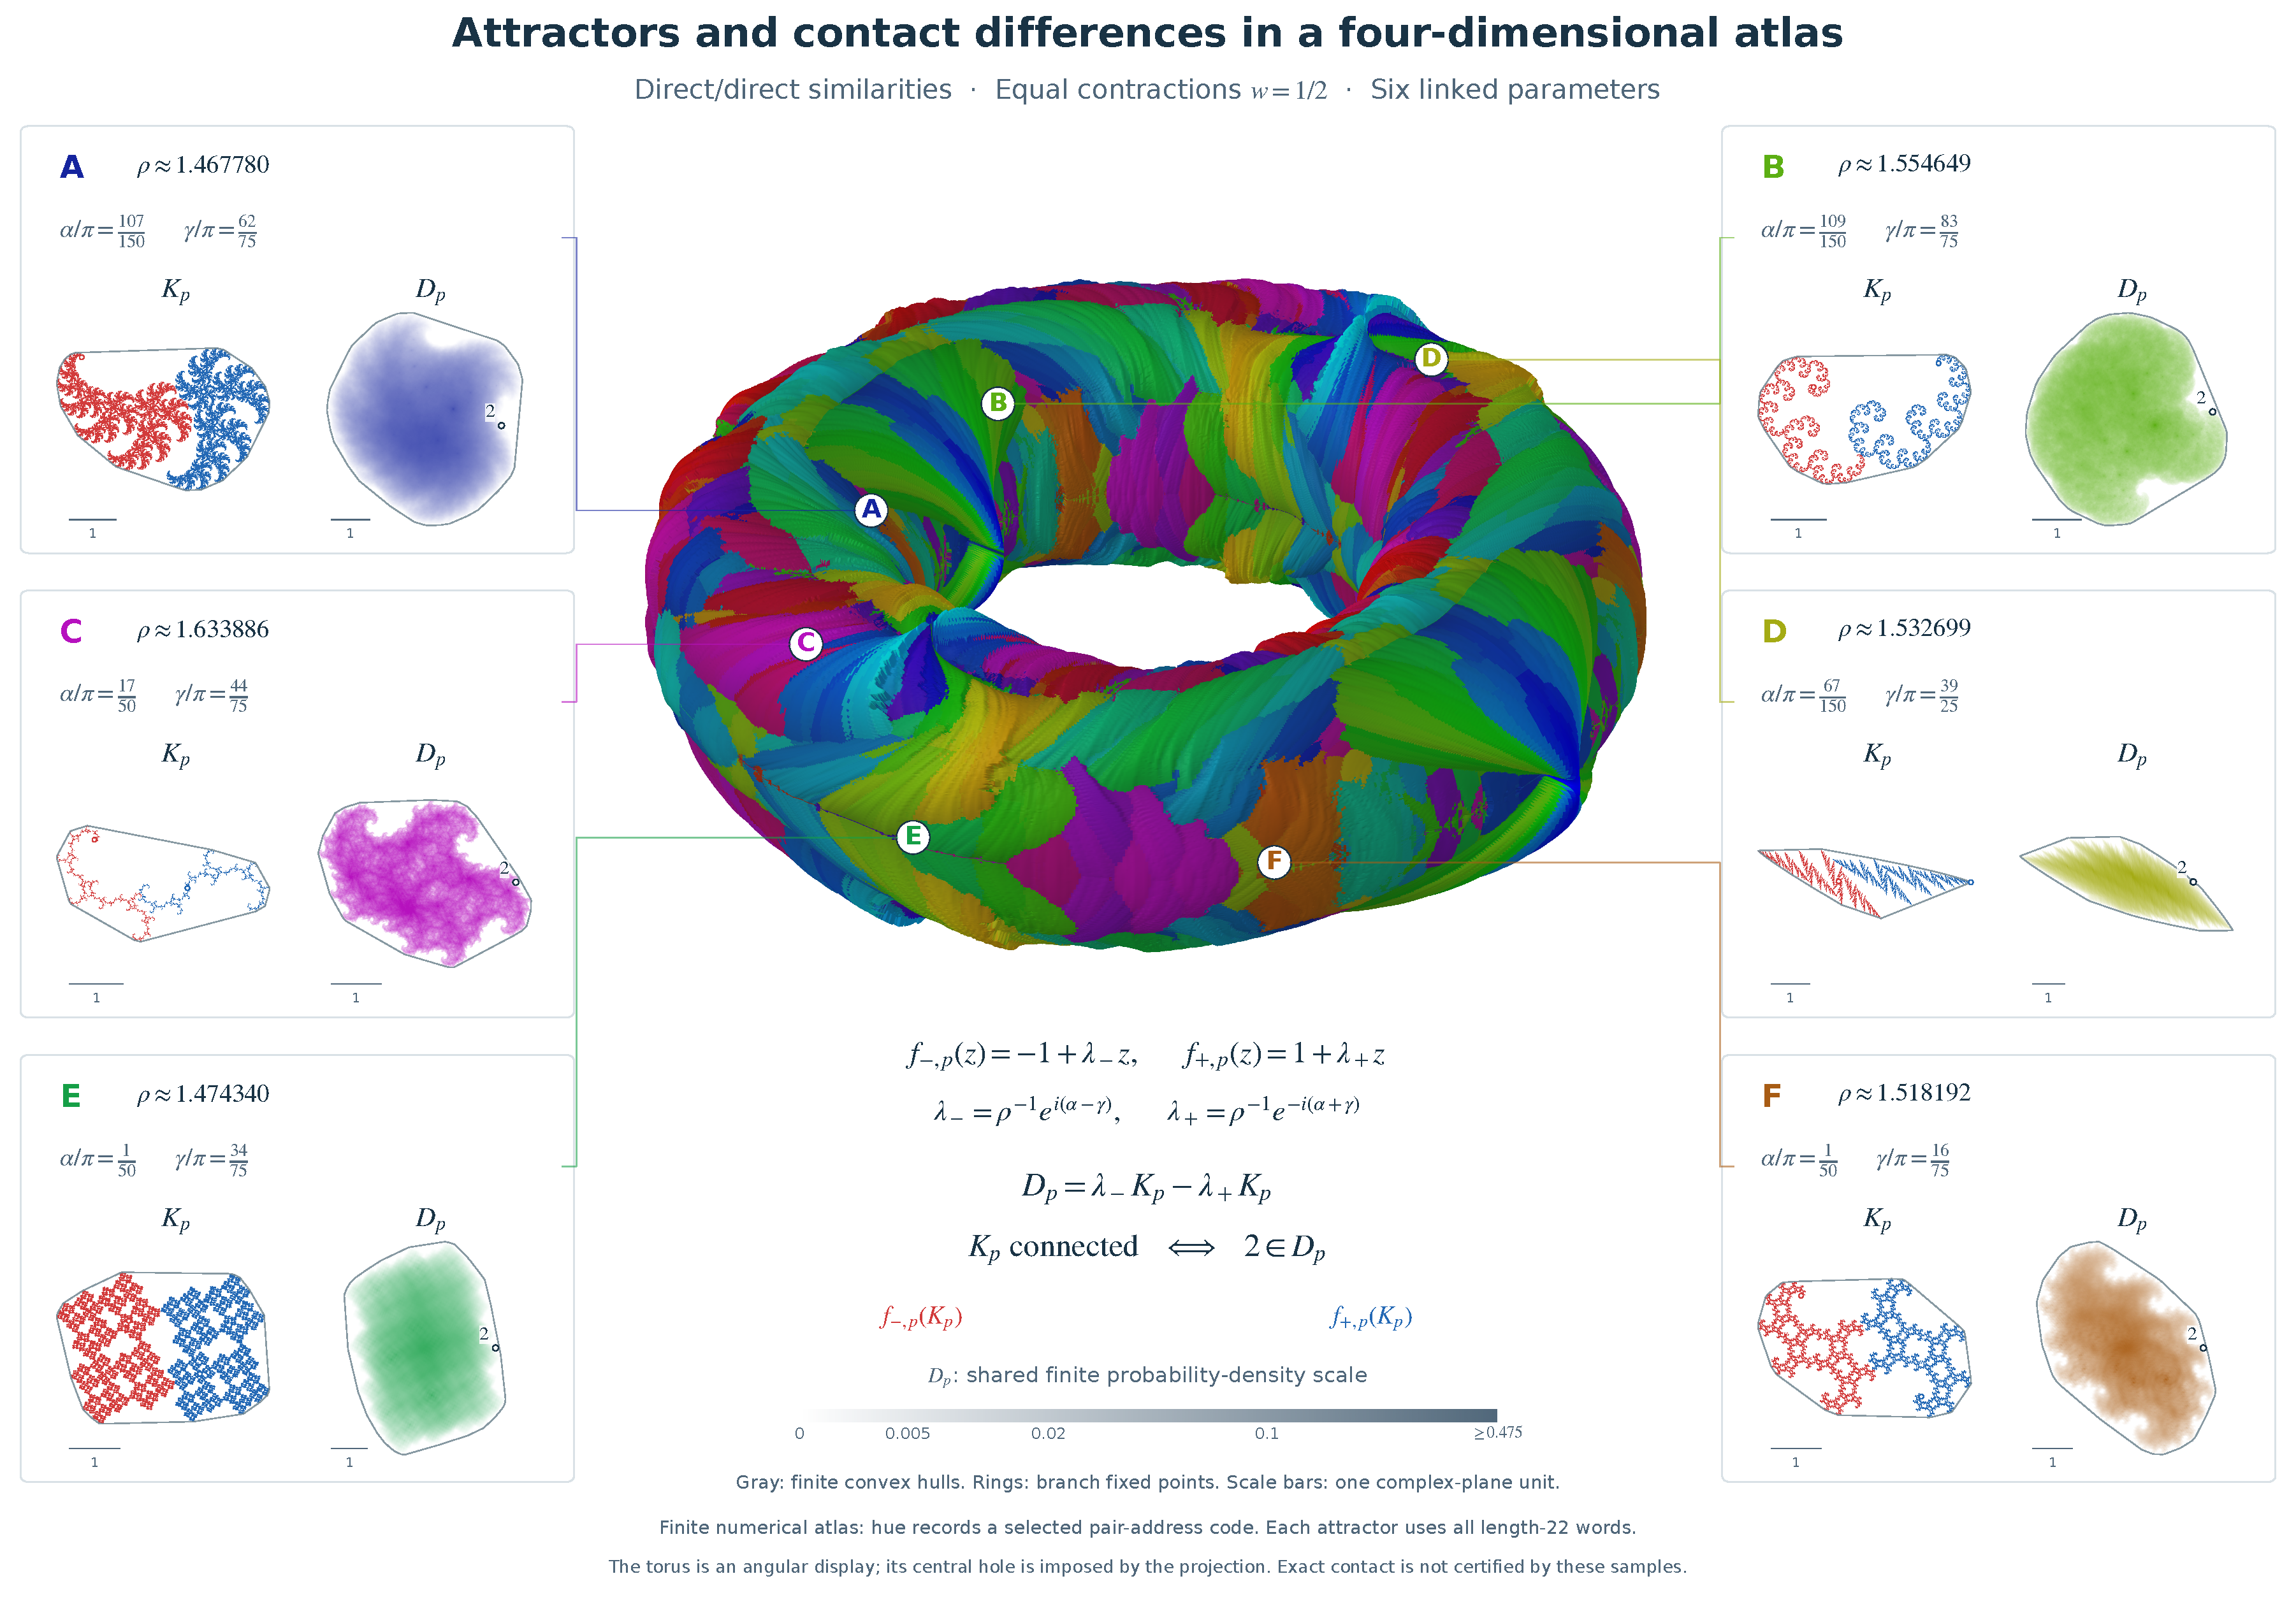
\includegraphics[width=.78\textwidth]{figures/atlas_hero.pdf}
\end{center}
\vspace{-.8cm}
\begin{columns}[t]
\separatorcolumn
\begin{column}{\colwidth}
\begin{block}{1. One atlas in exterior parameters}
Two complex parameters with $|c_1|,|c_2|>1$ define
\[
 S_1(z)=-1+c_1^{-1}J_{\kappa_1}(z),\qquad
 S_2(z)=1+c_2^{-1}J_{\kappa_2}(z),
\]
where $J_+(z)=z$ and $J_-(z)=\bar z$.
Direct/direct, direct/opposite and opposite/opposite maps give three orientation types.
For $K=S_1(K)\cup S_2(K)$, connectedness becomes
\[
 \boxed{\ 2\in c_1^{-1}J_{\kappa_1}(K)-c_2^{-1}J_{\kappa_2}(K)\ }.
\]
The atlas separates phases, magnitude and weight:
\[
 \rho=\frac{2|c_1||c_2|}{|c_1|+|c_2|},\qquad
 w=\frac{|c_2|}{|c_1|+|c_2|}.
\]
A three-dimensional angular projection shows the surfaces; colour records the fourth coordinate $w$.
\end{block}
\end{column}
\separatorcolumn
\begin{column}{\colwidth}
\begin{block}{2. Curve families inside the connectedness loci}
A binary zipper joins $0$ to $1$ through a vertex $q$.
Its plane orientation and endpoint reversal $(e_1,e_2)$ select a smooth two-dimensional surface inside the atlas.
Its stable set consists of embedded canonical curves:
\[
 \boxed{\ q\in\mathcal S_{\kappa,e}\ \Longleftrightarrow\ F_1(K_q)\cap F_2(K_q)=\{q\}\ }.
\]
Finite endpoint-return identities certify whole regions of stable parameters. These regions lie in the band
\[
 \boxed{\ 2\sqrt{w^2+(1-w)^2}<\rho\le2\ }.
\]
Below, four selected families share three parameter probes. The DD$(1,1)$ surface contains the Koch/wiggle island [3].
The exterior slice coordinate is $c=1/q$; both similarity parameters have modulus greater than one.
\end{block}
\end{column}
\separatorcolumn
\end{columns}
\vspace{.05cm}
\begin{center}
\begin{minipage}{.94\textwidth}
\begin{block}{3. Four stable surfaces, twelve linked curve examples}
\vspace{-.05cm}
{\centering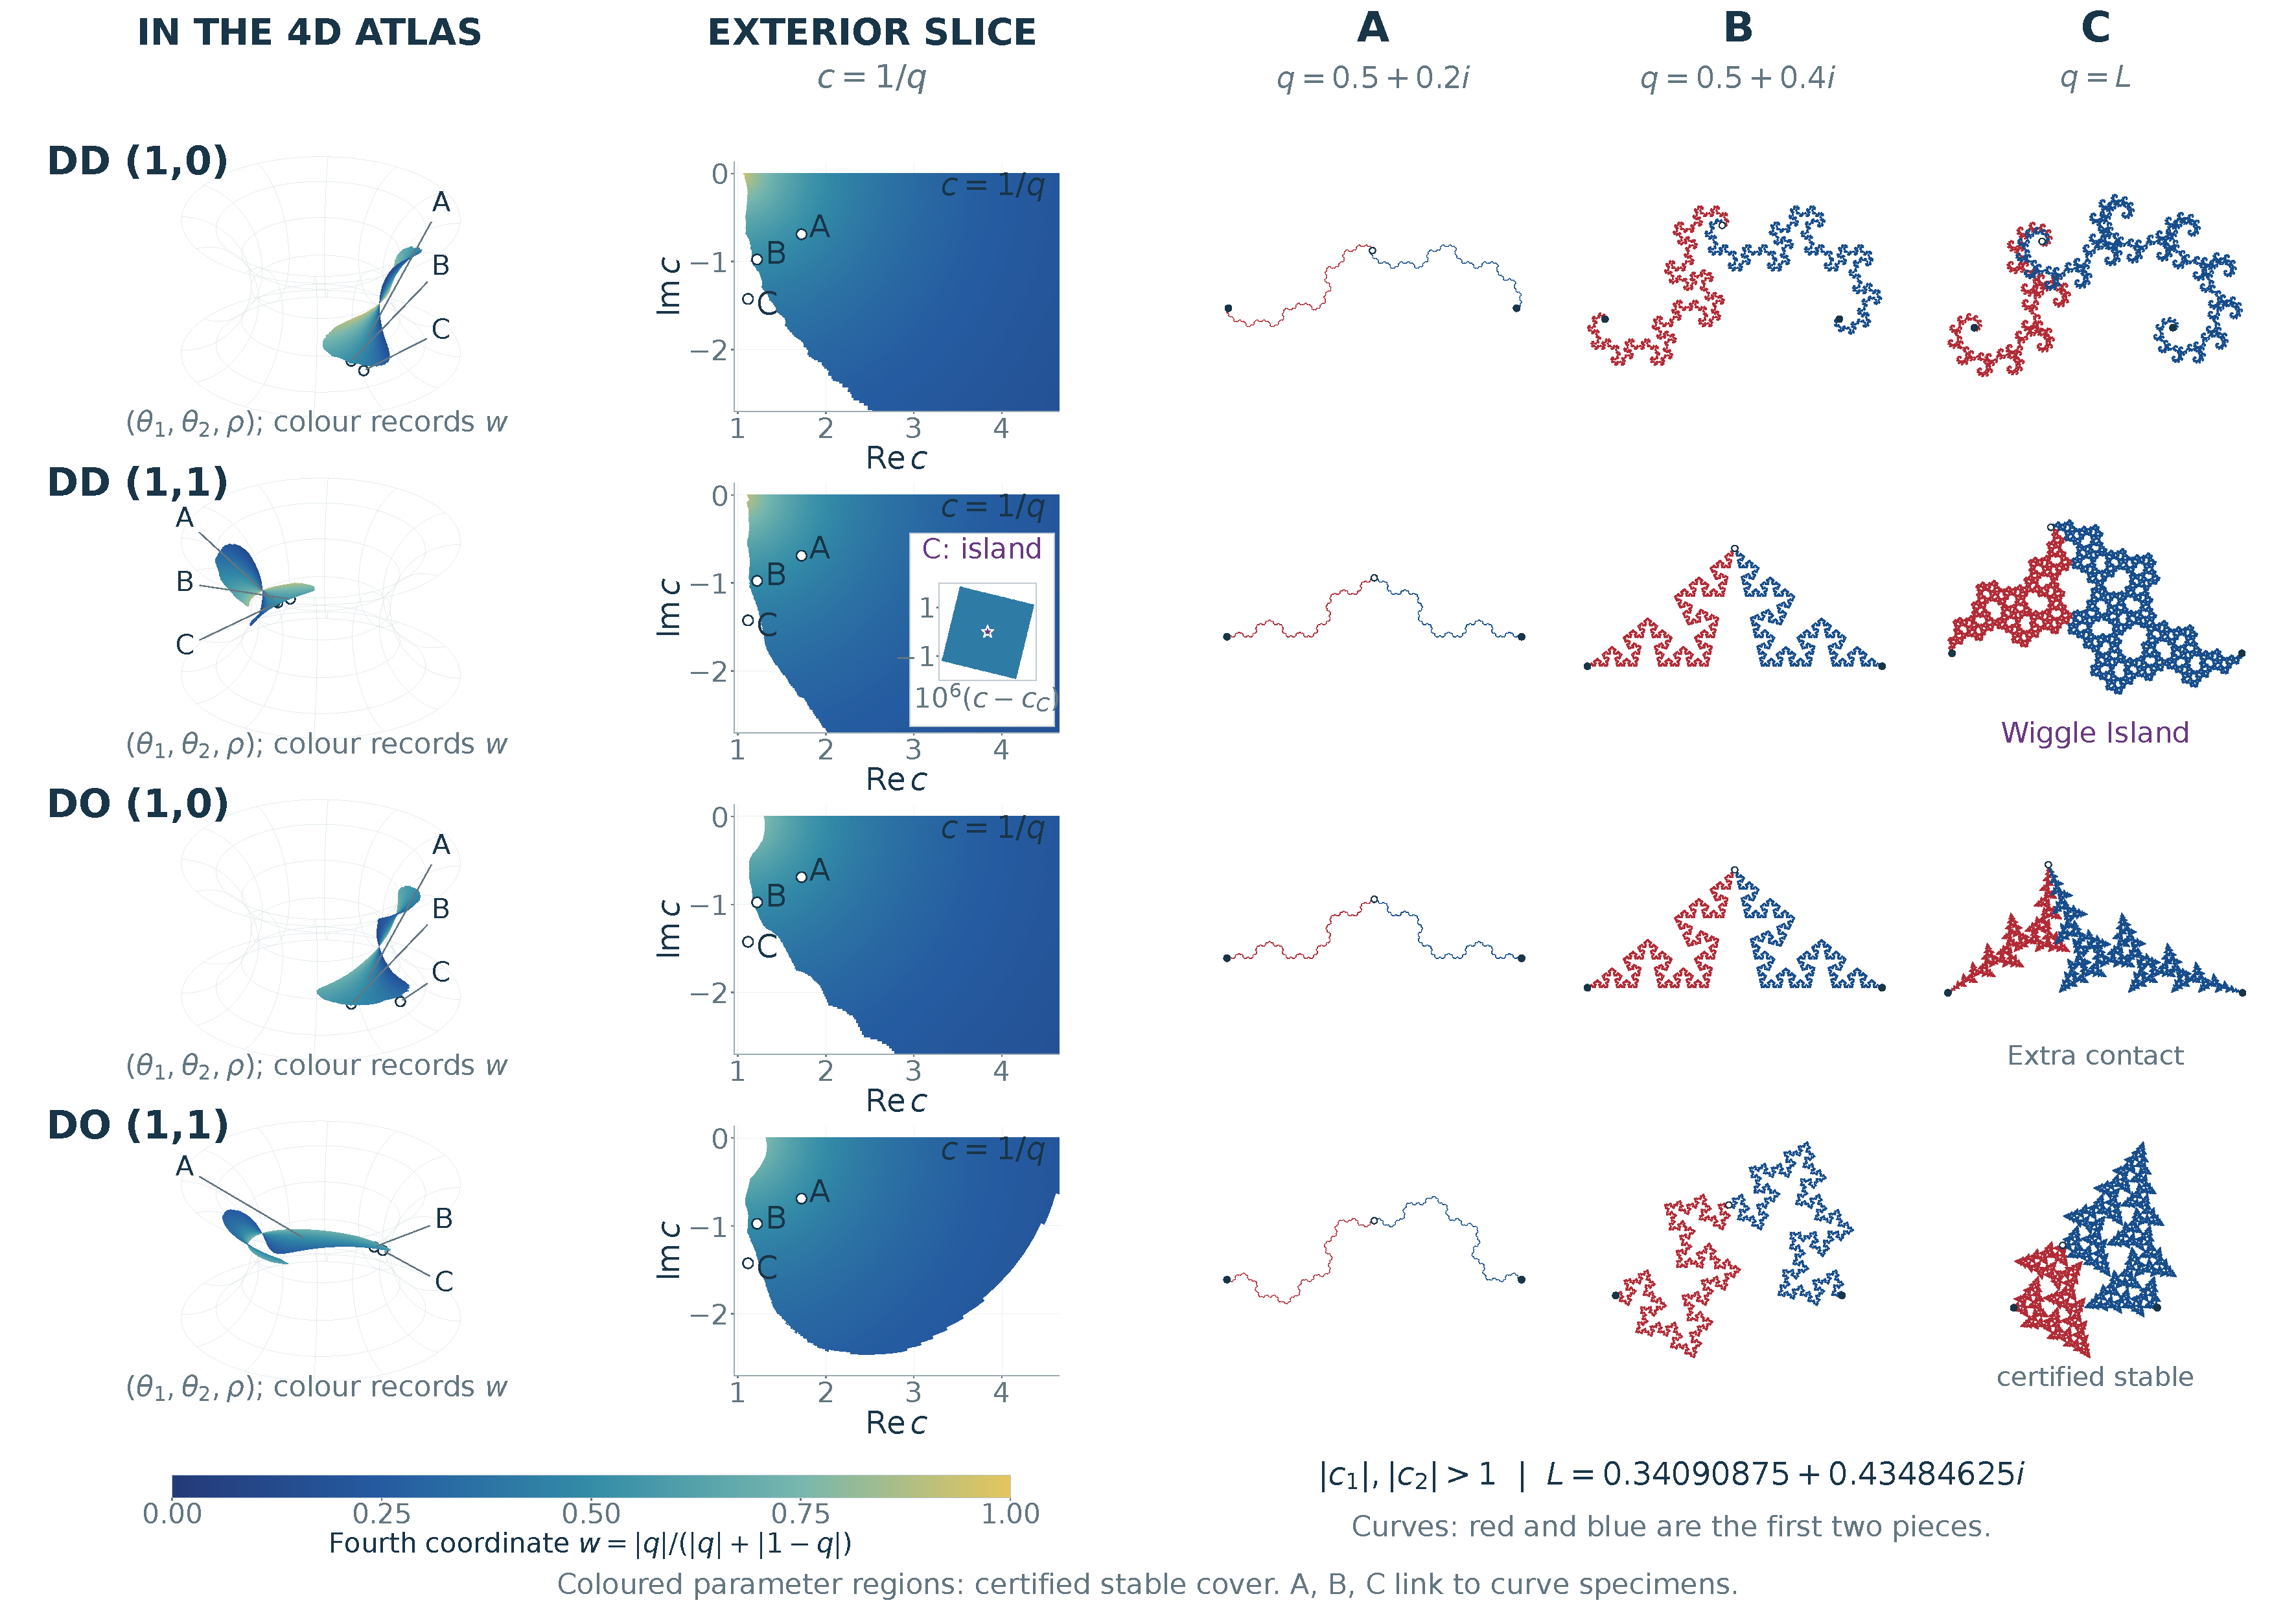
\includegraphics[width=\linewidth]{figures/four_family_poster.pdf}\par}
\end{block}
\vspace{.1cm}
\begin{center}
\href{https://complextrees.com/4D/}{\color{AtlasBlue}\fontsize{37}{43}\selectfont\bfseries Explore the atlas: complextrees.com/4D/}
\end{center}
{\fontsize{22}{28}\selectfont\color{AtlasGray}
Companion manuscript: B. Espigul\'e, \emph{Four-Dimensional Connectedness Loci and Structural Stability for Planar Binary Similarities} (2026).\par}
\vspace{.05cm}
{\fontsize{18}{22}\selectfont\color{AtlasGray}\setlength{\parskip}{2pt}
\textbf{References.} [1] B. Espigul\'e. \emph{Families of connected self-similar sets generated by complex trees}. arXiv:1902.11282 (2019).\par
[2] B. Espigul\'e Pons. \emph{Collinear Fractals and Connectedness Loci: Topology, Finite Capture, and Restricted Polynomial Roots}. Doctoral thesis (submitted), Universitat de Girona, 2026. \href{https://complextrees.com/research/thesis/}{complextrees.com/research/thesis/}.\par
[3] D. Calegari. \emph{Wiggle Island}. arXiv:2205.11442 (2022; revised 2026).\par
}
\vspace{.25cm}
{\color{AtlasBlue!25}\hrule height1pt}
\vspace{.25cm}
{\fontsize{20}{25}\selectfont\color{AtlasGray}
Supported by the Spanish Ministerio de Ciencia, Innovaci\'on y Universidades through project PID2023-146424NB-I00.\par}
\end{minipage}
\end{center}
\end{frame}
\end{document}
